\documentclass[DaoFP]{subfiles}
\begin{document}
    \setcounter{chapter}{9}

    \chapter{Adjunctions(伴随)}

    一位雕塑家通过去除不相关的石头直到雕塑显现出来。一位数学家通过抽象掉不相关的细节直到模式显现出来。

    我们能够使用映射入(mapping-in)和映射出(mapping-out)属性来定义许多构造。这些属性可以紧凑地表示为同态集(hom-sets)之间的同构关系。这种自然同构的模式被称为伴随(adjunction),一旦被识别出来,它几乎无处不在。

    \section{The Currying Adjunction(柯里化伴随)}

    指数对象(exponential)的定义是一个经典的伴随的例子,它关联了映射出和映射入的关系。每一个从积(product)出的映射对应于一个唯一的映射入指数对象:
    \[  \mathcal{C}(e \times a, b ) \cong  \mathcal{C} (e, b^a)  \]
    在左侧,$b$对象充当了焦点;在右侧,$e$对象成为了观察者。

    我们可以发现有两个函子(functors)在起作用。它们都以$a$为参数。在左侧,我们有积函子$(- \times a)$应用于$e$。在右侧,我们有指数函子$(-)^a$应用于$b$。

    如果我们将这些函子写作:
    \[ L_a e = e \times a \]
    \[ R_a b = b^a \]
    那么同态集之间的自然同构
    \[ \mathcal{C}(L_a e, b) \cong \mathcal{C}(e, R_a b) \]
    就被称为它们之间的伴随。

    在具体操作中,这个同构告诉我们,给定一个映射$\phi \in \mathcal{C}(L_a e, b)$,就有一个唯一的映射$\phi^T \in \mathcal{C}(e, R_a b)$,反之亦然。这些映射有时被称为彼此的\emph{转置}(transpose)——这个术语借用了矩阵代数的名称。

    伴随的简写为$L \dashv R$。将积函子代入$L$,将指数函子代入$R$,我们可以简洁地将柯里化伴随写为:

    \[ (- \times a) \dashv (-)^a \]

    指数对象$b^a$有时被称为\index{internal hom}\emph{内部同态},记作$[a, b]$。这与\emph{外部同态}相对,外部同态是集合$\cat C (a, b)$。外部同态\emph{不是} $\cat C$中的对象(除非$\cat C$本身是$\Set$)。使用这个记号,柯里化伴随可以写为:
    \[  \mathcal{C}(e \times a, b) \cong  \mathcal{C} (e, [a, b])  \]
    在这个伴随成立的范畴被称为笛卡尔封闭范畴(cartesian closed category)。

    由于函数在每种编程语言中都起着核心作用,因此笛卡尔封闭范畴构成了所有编程模型的基础。我们将指数$b^a$解释为函数类型$a \to b$。

    这里,$e$起着外部环境的作用——在λ演算中对应$\Gamma$。$\cat C(\Gamma \times a, b)$中的态射被解释为在环境$\Gamma$中扩展了一个类型为$a$的变量的表达式。函数类型$a \to b$因此表示一个闭包(closure),它可能从其环境中捕获一个类型为$e$的值。

    顺便说一句,(小)范畴的范畴$\mathbf{Cat}$也是笛卡尔封闭的,这在乘积范畴和函子范畴之间的伴随中得到了反映,并使用了相同的内部同态记号:
    \[ \mathbf{Cat} (\cat A \times \cat B, \cat C) \cong \mathbf{Cat} (\cat A, [\cat B, \cat C]) \]
    这里,两个同态集都是自然变换的集合。

    \section{The Sum and the Product Adjunctions(和与积的伴随)}

    柯里化伴随关联了两个自函子(endofunctors),但伴随可以很容易地推广到在不同范畴之间的函子。我们先来看看一些例子。

    \subsection{The Diagonal Functor(对角函子)}

    和(sum)与积(product)类型是使用双射(bijections)定义的,其中一侧是一个单一的箭头,另一侧是一对箭头。一对箭头可以看作是积范畴(product category)中的单一箭头。

    为了探索这一思想,我们需要定义对角函子(diagonal functor)$\Delta$,这是一个从$\mathcal{C}$到$\mathcal{C} \times \mathcal{C}$的特殊映射。它将一个对象$x$复制成一对对象$\langle x, x \rangle$。它也将一个箭头$f$复制为$\langle f, f \rangle$。

    有趣的是,对角函子与我们之前看到的常函子(constant functor)有关。常函子可以被视为一个有两个变量的函子——它只是忽略了第二个变量。我们在Haskell定义中见过:
    \begin{haskell}
        data Const c a = Const c
    \end{haskell}

    为了看到两者之间的联系,让我们将积范畴$\mathcal{C} \times \mathcal{C}$视为函子范畴$[\mathbf{2}, \mathcal{C}]$,换句话说,是$\mathbf{Cat}$中的指数对象$\mathcal{C}^{\mathbf{2}}$。实际上,从$\mathbf{2}$(带有两个对象的简图范畴)的函子选取了一对对象——这等同于积范畴中的单一对象。

    一个从$\mathcal{C}$到$[\mathbf{2}, \mathcal{C}]$的函子可以被展开为$\mathcal{C} \times \mathbf{2} \to \mathcal{C}$。对角函子忽略了来自$\mathbf{2}$的第二个参数:无论第二个参数是$1$还是$2$,它做的事情是一样的。这正是常函子所做的。因此,我们为它们都使用了相同的符号$\Delta$。

    顺便提一下,这种论证可以轻松推广到任何索引范畴,而不仅仅是$\mathbf{2}$。

    \subsection{The Sum Adjunction(和伴随)}

    回想一下,和是通过其映射出属性定义的。$a + b$的所有箭头与分别从$a$和$b$出来的一对箭头一一对应。用同态集的术语,我们可以写成:
    \[  \mathcal{C} (a + b, x) \cong \mathcal{C}( a , x) \times \mathcal{C}( b , x)\]
    这里右边的乘积只是集合的笛卡尔乘积,即对的集合。此外,我们之前已经看到,这种双射在$x$上是自然的。

    我们知道一对箭头在积范畴中是一个单一箭头。因此,我们可以将右边的元素看作是在$\mathcal{C} \times \mathcal{C}$中的箭头,从对象$\langle a, b \rangle$到对象$\langle x, x \rangle$。后者可以通过对$x$作用的对角函子$\Delta$获得。我们有:

    \[  \mathcal{C} (a + b, x) \cong (\mathcal{C} \times \mathcal{C})( \langle a, b \rangle , \Delta x)\]
    这是两个不同范畴中同态集之间的双射。它满足自然性条件,因此它是一个自然同构。

    我们还可以在这里发现一对函子。在左边,我们有一个函子,它接受一对对象$\langle a, b \rangle$并生成它们的和$a + b$:
    \[ (+) \colon \mathcal{C} \times \mathcal{C} \to \mathcal{C}\]
    在右边,我们有对角函子$\Delta$,它朝相反的方向运行:
    \[ \Delta \colon \mathcal{C} \to  \mathcal{C} \times \mathcal{C} \]
    总之,我们有两个范畴之间的一对函子:
    \[
        \begin{tikzcd}
            \mathcal{C}
            \arrow[rr, bend right, "\Delta"']
            &&
            \mathcal{C} \times \mathcal{C}
            \arrow[ll, bend right, "(+)"']
        \end{tikzcd}
    \]
    以及同态集之间的同构:
    \[
        \begin{tikzcd}
            a + b
            \arrow[d, bend right, red, dashed]
            \arrow[d, dashed]
            \arrow[d, bend left, blue, dashed]
            &&
            \langle a , b \rangle
            \arrow[d, bend right, red, dashed]
            \arrow[d, dashed]
            \arrow[d, bend left, blue, dashed]
            \arrow[ll, bend right, "(+)"']
            \\
            x
            \arrow[rr, bend right, "\Delta"']
            &&
            \langle x, x \rangle
        \end{tikzcd}
    \]
    换句话说,我们有了伴随关系:
    \[ (+) \dashv \Delta \]

    \subsection{The Product Adjunction(积伴随)}

    我们可以将相同的推理应用于积的定义。这次我们有一个自然同构,关联的是一对箭头和一个映射入积。

    \[  \mathcal{C} (x, a) \times \mathcal{C}(x, b) \cong  \mathcal{C} (x, a \times b)  \]
    将一对箭头替换为积范畴中的箭头,我们得到:

    \[  (\mathcal{C} \times \mathcal{C})( \Delta x,  \langle a, b \rangle ) \cong  \mathcal{C} (x, a \times b)  \]
    这就是朝着相反方向运行的两个函子:
    \[
        \begin{tikzcd}
            \mathcal{C} \times \mathcal{C}
            \arrow[rr, bend right, "(\times)"']
            &&
            \mathcal{C}
            \arrow[ll, bend right, "\Delta"']
        \end{tikzcd}
    \]
    以及同态集之间的同构:

    \[
        \begin{tikzcd}
            \langle x, x \rangle
            \arrow[d, bend right, red, dashed]
            \arrow[d, dashed]
            \arrow[d, bend left, blue, dashed]
            &&
            x
            \arrow[d, bend right, red, dashed]
            \arrow[d, dashed]
            \arrow[d, bend left, blue, dashed]
            \arrow[ll, bend right, "\Delta"']
            \\
            \langle a , b \rangle
            \arrow[rr, bend right, "(\times)"']
            &&
            a \times b
        \end{tikzcd}
    \]
    换句话说,我们有了伴随关系:
    \[ \Delta \dashv (\times) \]

    \subsection{Distributivity(分配律)}

    在双笛卡尔封闭范畴(bicartesian closed category)中,积分配于和。我们已经使用通用构造看到了证明的一种方向。结合Yoneda引理,伴随关系给了我们更强大的工具来解决这个问题。

    我们希望证明以下自然同构:
    \[(b + c) \times a \cong b \times a + c \times a \]
    与其直接证明这个等式,我们将展示从两边映射出的所有映射到任意对象$x$是同构的:
    \[  \mathcal{C} ((b + c) \times a, x) \cong \mathcal{C}(b \times a + c \times a, x) \]
    左边是从积映射出,因此我们可以将柯里化伴随应用于它:
    \[  \mathcal{C} ((b + c) \times a, x) \cong \mathcal{C}(b + c, x^a) \]
    这给了我们一个从和映射出的映射,根据和伴随,它与两个映射的乘积同构:
    \[  \mathcal{C}(b + c, x^a) \cong \mathcal{C}(b, x^a) \times \mathcal{C}(c, x^a)\]
    现在我们可以对两个分量应用柯里化伴随的逆映射:
    \[  \mathcal{C}(b, x^a) \times \mathcal{C}(c, x^a) \cong \mathcal{C}(b \times a, x) \times \mathcal{C}(c \times a, x)\]
    使用和伴随的逆映射,我们得到最终结果:
    \[ \mathcal{C}(b \times a, x) \times \mathcal{C}(c \times a, x) \cong \mathcal{C}(b \times a + c \times a, x) \]

    这个证明中的每一步都是自然同构,因此它们的组合也是自然同构。通过Yoneda引理,分配律左侧和右侧形成的两个对象因此是同构的。

    这一陈述的一个更短的证明来自我们即将讨论的左伴随的性质。

    \section{Adjunction between Functors(函子之间的伴随)}

    通常,伴随关联了两个在两个范畴之间的相反方向的函子。左函子为
    \[ L \colon \mathcal{D} \to \mathcal{C}\]
    右函子为:
    \[ R \colon \mathcal{C} \to  \mathcal{D} \]
    伴随$L \dashv R$定义为两个同态集之间的自然同构。
    \[  \mathcal{C} (L x, y) \cong \mathcal{D}( x , R y)\]
    换句话说,我们有一组在$x$和$y$上自然的可逆函数集:
    \[ \phi_{x y} \colon  \mathcal{C} (L x, y) \to \mathcal{D}( x , R y) \]
    例如,$y$上的自然性意味着,对于任意$f \colon y \to y'$,下图是交换的:
    \[
        \begin{tikzcd}
            \mathcal{C}(L x, y)
            \arrow[d, leftrightarrow, "\phi_{x y}"]
            \arrow[r, "{\mathcal{C}(L x, f)}"]
            &
            \mathcal{C}(L x, y')
            \arrow[d, leftrightarrow, "\phi_{x y'}"]
            \\
            \mathcal{D}(x, R y)
            \arrow[r, "{\mathcal{D}(x, R f)}"]
            & \mathcal{D}(x, R y')
        \end{tikzcd}
    \]
    或者,考虑到同态函子的箭头提升与后合成(post-composition)相同:
    \[
        \begin{tikzcd}
            \mathcal{C}(L x, y)
            \arrow[d, leftrightarrow, "\phi_{x y}"]
            \arrow[r, "f \circ -"]
            &
            \mathcal{C}(L x, y')
            \arrow[d, leftrightarrow, "\phi_{x y'}"]
            \\
            \mathcal{D}(x, R y)
            \arrow[r, "R f \circ -"]
            & \mathcal{D}(x, R y')
        \end{tikzcd}
    \]
    双头箭头可以沿任意方向(使用$\phi^{-1}_{x y}$向上)遍历,因为它们是同构的组成部分。

    图示上,我们有两个函子:
    \[
        \begin{tikzcd}
            \mathcal{C}
            \arrow[rr, bend right, "R"']
            &&
            \mathcal{D}
            \arrow[ll, bend right, "L"']
        \end{tikzcd}
    \]
    并且,对于任意一对$x$和$y$,两个同构的同态集:
    \[
        \begin{tikzcd}
            L x
            \arrow[d, bend right, red, dashed]
            \arrow[d, dashed]
            \arrow[d, bend left, blue, dashed]
            &&
            x
            \arrow[d, bend right, red, dashed]
            \arrow[d, dashed]
            \arrow[d, bend left, blue, dashed]
            \arrow[ll, bend right, "L"']
            \\
            y
            \arrow[rr, bend right, "R"']
            &&
            R y
        \end{tikzcd}
    \]
    这些同态集来自两个不同的范畴,但集合就是集合。我们说$L$是$R$的左伴随,或者$R$是$L$的右伴随。

    在Haskell中,这可以简化为一个多参数类型类:
    \begin{haskell}
        class (Functor left, Functor right) => Adjunction left right where
        ltor :: (left x -> y) -> (x -> right y)
        rtol :: (x -> right y) -> (left x -> y)
    \end{haskell}
    在文件顶部需要以下指示:
    \begin{haskell}
    {-# language MultiParamTypeClasses #-}
    \end{haskell}

    因此,在双笛卡尔范畴中,和是对角函子的左伴随;积是其右伴随。我们可以非常简洁地写出这一关系(或者我们可以将其印在粘土中,作为楔形文字的现代版本):
    \[ (+) \dashv \Delta \dashv (\times) \]

    \begin{exercise}
        绘制见证伴随函数$\phi_{x y}$在$x$上自然性的交换图。
    \end{exercise}

    \begin{exercise}
        伴随公式左侧的同态集$\mathcal{C} (L x, y)$暗示$L x$可以被视为某个函子(共预层)的表示对象。这个函子是什么?提示:它将$y$映射到一个集合。这个集合是什么?
    \end{exercise}

    \begin{exercise}
        相应地,表示对象$a$对于预层$P$的定义是:
        \[P x \cong \mathcal{D}(x, a)\]
        在伴随公式中,$R y$是哪个预层的表示对象。
    \end{exercise}

    \section{Limits and Colimits as Adjunctions(极限与余极限作为伴随)}

    极限的定义也涉及同态集之间的自然同构:
    \[ [\cat J, \mathcal{C}](\Delta_x, D)  \cong \mathcal{C}(x, \text{Lim} D) \]
    左侧的同态集在函子范畴中。其元素是锥(cones),即常函子$\Delta_x$和图示函子$D$之间的自然变换。右侧的是$\mathcal{C}$中的同态集。

    在一个所有极限都存在的范畴中,我们有这两个函子之间的伴随:
    \[ \Delta_{(-)} \colon \mathcal{C} \to  [\cat J, \mathcal{C}] \]
    和:
    \[ \text{Lim}{(-)} \colon  [\cat J, \mathcal{C}] \to \mathcal{C} \]

    相应地,余极限由以下自然同构描述:
    \[ [\cat J, \mathcal{C}](D, \Delta_x)  \cong \mathcal{C}( \text{Colim} D, x) \]
    我们可以用一个简洁的公式表示这两个伴随:
    \[ \text{Colim} \dashv \Delta \dashv \text{Lim}\]

    特别地,由于积范畴$\cat C \times \cat C$等价于$\cat C^2$,或者函子范畴$[\mathbf{2}, \cat C]$,我们可以将积和余积重新表述为极限和余极限:
    \[ [\mathbf{2}, \cat C](\Delta_x, \langle a, b \rangle) \cong \cat C(x, a \times b) \]
    \[ \cat C( a + b, x) \cong [\mathbf{2}, \cat C]( \langle a, b \rangle, \Delta_x) \]
    这里$\langle a, b \rangle$表示一个图示,这是一个函子$D \colon \mathbf{2} \to \cat C$作用于$\mathbf{2}$的两个对象。

    \section{Unit and Counit of an Adjunction(伴随的单位元与伴随元)}

    我们通过比较箭头的相等性来比较它们,但我们更喜欢使用同构来比较对象。

    然而,当涉及到函子时,我们却遇到了问题。一方面,它们是函子范畴中的对象,因此同构是比较的方式;但另一方面,它们在$\mathbf{Cat}$中是箭头,所以可能直接比较它们的相等性也没什么问题?

    为了更清楚地理解这一困境,我们应该问自己\emph{为什么}我们要使用箭头的相等性。并不是因为我们喜欢相等性,而是因为在一个集合中,除了比较元素是否相等之外,我们无事可做。同态集中的两个元素要么相等要么不相等,仅此而已。

    但在$\mathbf{Cat}$中情况并非如此,正如我们所知,它是一个$2$-范畴。这里,同态集本身具有范畴的结构——即函子范畴。在$2$-范畴中,我们有箭头之间的箭头,因此特别地,我们可以定义箭头之间的同构。在$\mathbf{Cat}$中,这些同构就是函子之间的自然同构。

    然而,尽管我们有选择使用同构代替箭头相等性的选项,但$\mathbf{Cat}$中的范畴法则仍然表示为相等性。例如,函子$F$与恒等函子的复合是\emph{等于}$F$的,同样地,结合律也是如此。如果$2$-范畴中的法则严格满足,那么它被称为\emph{严格的}(strict),而$\mathbf{Cat}$就是一个严格$2$-范畴的例子。

    但就比较范畴而言,我们有更多的选择。范畴是$\mathbf{Cat}$中的对象,因此有可能将两个范畴的同构定义为一对函子$L$和$R$:
    \[
        \begin{tikzcd}
            \mathcal{C}
            \arrow[rr, bend right, "R"']
            \arrow[loop, "\text{Id}_{ \mathcal{C}} "']
            &&
            \mathcal{D}
            \arrow[ll, bend right, "L"']
            \arrow[loop, "\text{Id}_{ \mathcal{D}} "']
        \end{tikzcd}
    \]
    使得:
    \begin{align*}
        L \circ R = \text{Id}_{ \mathcal{C}} \\
        \text{Id}_{ \mathcal{D}} = R \circ L
    \end{align*}
    这个定义涉及函子的相等性。然而更糟糕的是,作用在对象上时,它涉及到对象的相等性:
    \begin{align*}
        L (R x) = x \\
        y = R (L y)
    \end{align*}
    这就是为什么更适合讨论一种更弱的范畴\emph{等价}(equivalence)的概念,其中相等性被替换为同构:
    \begin{align*}
        L \circ R \cong \text{Id}_{ \mathcal{C}} \\
        \text{Id}_{ \mathcal{D}} \cong R \circ L
    \end{align*}
    对于对象而言,范畴的等价意味着一个往返生成的对象与原始对象是同构的,而不是相等的。在大多数情况下,这正是我们所需要的。

    伴随也定义为一对相反方向的函子,因此有必要问一下往返的结果是什么。

    定义伴随的同构适用于任何一对对象$x$和$y$
    \[  \mathcal{C} (L x, y) \cong \mathcal{D}( x , R y)\]
    因此,特别地,如果我们将$y$替换为$L x$,那么我们得到:
    \[  \mathcal{C} (L x, L x) \cong \mathcal{D}( x , R (L x))\]
    我们现在可以使用Yoneda技巧,并在左侧选择恒等箭头$id_{L x}$。该同构将其映射到右侧的一个唯一箭头,我们将其称为$\eta_x$:
    \[ \eta_x \colon x \to R ( L x) \]
    不仅为每个$x$定义了这个映射,而且它在$x$上是自然的。自然变换$\eta$被称为伴随的\emph{单位元}(unit)。如果我们注意到左侧的$x$是恒等函子对$x$的作用,那么我们可以写成:
    \[ \eta \colon \text{Id}_{\mathcal{D}} \to R \circ L \]

    作为一个例子,我们来计算余积伴随的单位元:
    \[  \mathcal{C} (a + b, x) \cong (\mathcal{C} \times \mathcal{C})( \langle a, b \rangle , \Delta x)\]
    通过将$x$替换为$a + b$。我们得到:
    \[ \eta_{\langle a, b \rangle} \colon \langle a, b \rangle \to \Delta(a + b) \]
    这是一对箭头,它们正是两个注入$\langle \text{Left}, \text{Right} \rangle$。

    我们可以通过将$x$替换为$R y$来做一个类似的操作:
    \[  \mathcal{C} (L (R y), y) \cong \mathcal{D}( R y , R y)\]
    对应于右侧的恒等箭头,我们在左侧得到一个箭头:
    \[ \varepsilon_y \colon L (R y) \to y \]
    这些箭头形成了另一个自然变换,称为伴随的\emph{伴随元}(counit):
    \[ \varepsilon \colon L \circ R \to \text{Id}_{\mathcal{C}}  \]

    请注意,如果这两个自然变换是可逆的,它们将证明范畴的等价性。但即使它们不是,这种“半等价”在范畴论的上下文中仍然非常有趣。

    作为一个例子,我们来计算积伴随的伴随元:
    \[  (\mathcal{C} \times \mathcal{C})( \Delta x,  \langle a, b \rangle ) \cong  \mathcal{C} (x, a \times b)  \]
    通过将$x$替换为$a \times b$。我们得到:
    \[ \varepsilon_{\langle a, b \rangle} \colon \Delta (a \times b) \to \langle a, b \rangle \]
    这是一对箭头,它们正是两个投影$\langle \text{fst}, \text{snd} \rangle$。

    \begin{exercise}
        推导出余积伴随的伴随元和积伴随的单位元。
    \end{exercise}

    \subsection{Triangle Identities(三角恒等式)}

    我们可以使用单位元/伴随元对来形成伴随的一个等价定义。为此,我们首先从一对自然变换开始:
    \begin{align*}
        \eta \colon \text{Id}_{\mathcal{D}} \to R \circ L \\
        \varepsilon \colon L \circ R \to \text{Id}_{\mathcal{C}}
    \end{align*}
    并施加额外的\emph{三角恒等式}(triangle identities)。

    这些恒等式可以从伴随的标准定义推导出来,通过注意到$\eta$可以用来用复合$R \circ L$替换恒等函子,实际上让我们可以在任何适用恒等函子的地方插入$R \circ L$。

    类似地,$\varepsilon$可以用来消除复合$L \circ R$(即,将其替换为恒等)。

    因此,例如,从$L$开始:
    \[ L = L \circ \text{Id}_{\mathcal{D}} \xrightarrow{L \circ \eta} L \circ R \circ L \xrightarrow{\varepsilon \circ L} \text{Id}_{\mathcal{C}} \circ L = L \]
    在这里,我们使用了自然变换的水平组合,其中之一是恒等变换(也称为whiskering)。

    第一个三角恒等式是这种变换链结果为恒等自然变换的条件。图示上:

    \[
        \begin{tikzcd}
            L
            \arrow[r, "L \circ \eta"]
            \arrow[rd, "id_L"']
            & L \circ R \circ L
            \arrow[d, "\varepsilon \circ L"]
            \\
            & L
        \end{tikzcd}
    \]

    类似地,我们希望以下自然变换链也组合成恒等式:
    \[ R = \text{Id}_{\mathcal{D}} \circ R \xrightarrow{\eta \circ R} R \circ L \circ R \xrightarrow{R \circ \varepsilon} R \circ \text{Id}_{\mathcal{C}} = R \]
    或者,图示上:
    \[
        \begin{tikzcd}
            R
            \arrow[r, "\eta \circ R"]
            \arrow[rd, "id_R"']
            & R \circ L \circ R
            \arrow[d, "R \circ \varepsilon"]
            \\
            & R
        \end{tikzcd}
    \]

    事实证明,伴随还可以用满足三角恒等式的两个自然变换$\eta$和$\varepsilon$来定义:
    \begin{align*}
    (\varepsilon \circ L) \cdot (L \circ \eta) = id_L \\
    (R \circ \varepsilon) \cdot (\eta \circ R) = id_R
    \end{align*}

    通过这些, 可以很容易地恢复同态集的映射。例如,从箭头$f \colon x \to R y$开始,它是$\mathcal{D}( x , R y)$的一个元素。我们可以将其提升为
    \[L f \colon L x \to L (R y)\]
    然后我们可以使用$\eta$来将复合$L \circ R$压缩为恒等。结果是一个箭头$L x \to y$,它是$ \mathcal{C} (L x, y)$的一个元素。

    使用单位元和伴随元的伴随定义更加通用,因为它可以翻译到任意$2$-范畴设置。

    \begin{exercise}
        给定一个箭头$g \colon L x \to y$,使用$\varepsilon$和$R$是一个函子的事实来实现一个箭头$x \to R y$。提示:从对象$x$开始,看看你可以如何通过一个中途站到达$R y$。
    \end{exercise}

    \subsection{The Unit and Counit of the Currying Adjunction(柯里化伴随的单位元与伴随元)}

    让我们计算柯里化伴随的单位元和伴随元:
    \[  \mathcal{C}(e \times a, b ) \cong  \mathcal{C} (e, b^a)  \]
    如果我们将$b$替换为$e \times a$,我们得到
    \[  \mathcal{C}(e \times a, e \times a ) \cong  \mathcal{C} (e, (e \times a)^a)  \]
    对应于左侧的恒等箭头,我们在右侧得到了伴随的单位元:
    \[ \eta \colon e \to (e \times a)^a \]
    这是一个积构造器的柯里化版本。在Haskell中,我们将其写为:
    \begin{haskell}
        unit :: e -> (a -> (e, a))
        unit = curry id
    \end{haskell}

    伴随元更有趣。将$e$替换为$b^a$,我们得到:
    \[  \mathcal{C}(b^a \times a, b ) \cong  \mathcal{C} (b^a, b^a)  \]
    对应于右侧的恒等箭头,我们得到:
    \[ \varepsilon \colon b^a \times a \to b \]
    这就是函数应用箭头。

    在Haskell中:
    \begin{haskell}
        counit :: (a -> b, a) -> b
        counit = uncurry id
    \end{haskell}

    当伴随发生在两个自函子之间时,我们可以使用单位元和伴随元写一个替代的Haskell定义:
    \begin{haskell}
        class (Functor left, Functor right) =>
        Adjunction left right | left -> right, right -> left where
        unit   :: x -> right (left x)
        counit :: left (right x) -> x
    \end{haskell}
    另外的两个子句\hask{left -> right}和\hask{right -> left}告诉编译器,在使用伴随实例时,一个函子可以从另一个推导出来。这个定义需要以下编译扩展:
    \begin{haskell}
    {-# language MultiParamTypeClasses #-}
    {-# LANGUAGE FunctionalDependencies #-}
    \end{haskell}

    构成柯里化伴随的两个函子可以写成:
    \begin{haskell}
        data L r x = L (x, r)    deriving (Functor, Show)
        data R r x = R (r -> x)  deriving Functor
    \end{haskell}
    以及柯里化的\hask{Adjunction}实例:
    \begin{haskell}
        instance Adjunction (L r) (R r) where
        unit x = R (\r -> L (x, r))
        counit (L (R f, r)) = f r
    \end{haskell}
    第一个三角恒等式声明以下多态函数:
    \begin{haskell}
        triangle :: L r x -> L r x
        triangle = counit . fmap unit
    \end{haskell}
    是恒等的,第二个也是:
    \begin{haskell}
        triangle' :: R r x -> R r x
        triangle' = fmap counit . unit
    \end{haskell}
    注意,这两个函数需要使用功能依赖才能正确定义。三角恒等式无法在Haskell中表达,因此实现伴随的开发人员必须自己证明它们。
    \begin{exercise}
        测试柯里化伴随的第一个三角恒等式的一些例子。以下是一个例子:
        \begin{haskell}
            triangle (L (2, 'a'))
        \end{haskell}
    \end{exercise}

    \begin{exercise}
        你会如何测试柯里化伴随的第二个三角恒等式?提示:\hask{triangle'}的结果是一个函数,所以你无法直接显示它,但你可以调用它。
    \end{exercise}

    \section{Adjunctions Using Universal Arrows}

We've seen the definition of an adjunction using the isomorphism of hom-sets, and another one using the pair of unit/counit. It turns out that we can define an adjunction using just one element of this pair, as long as it satisfies certain universality condition. To see that, we will construct a new category whose objects are arrows. 

We've seen before an example of such a category---the slice category $\cat C/ c$ that collects all the arrows that converge on $c$. Such a category describes the view of the object $c$ from every possible angle in $\cat C$. 

\subsection{Comma category}
When dealing with an adjunction:
\[  \mathcal{C} (L d, c) \cong \mathcal{D}( d , R c)\]
we are observing the object $c$ from a narrower perspective defined by the functor $L$. Think of $L$ as defining a model of the category $\cat D$ inside $\cat C$. We are interested in the view of $c$ from the perspective of this model. The arrows that describe this view form the comma category $L/c$.


\[
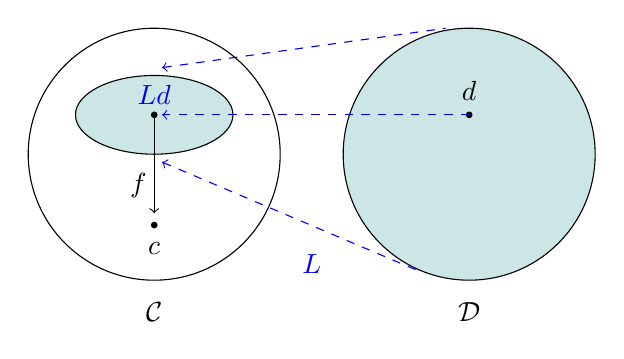
\begin{tikzpicture}
  \def\Xa{2.0};
  \def\Xb{-2.0};
  
  \def\Ytip{-0.9};
  \def\Yo{0.5}; % oval
  \def\Yb{-2.0}; % labels
         \draw (\Xa, 0)[fill=blue!50!green!20]  ellipse (1.6 and 1.6);
         \draw (\Xb , 0) ellipse (1.6 and 1.6);
         % oval
         \draw (\Xb , \Yo)[fill=blue!50!green!20] ellipse (1 and 0.5);
         
        % apex
        \filldraw (\Xb, \Ytip) circle (1pt);
        \node at ( \Xb, \Ytip - 0.3) { $c$ };
        
        % image
        \filldraw (\Xa, \Yo) circle (1pt);
        \node at ( \Xa, \Yo + 0.3) { $d$ };
        
	% middle of the cone
	\draw[->] (\Xb, \Yo) -- (\Xb, \Ytip + 0.15);
	\node at (\Xb - 0.2, \Ytip + 0.5) {$f$};
        	% sides of the cone
	%\draw (\Xb, \Ytip) -- (\Xb + 0.95, \Yo - 0.15);
	%\draw (\Xb, \Ytip) -- (\Xb - 0.95, \Yo - 0.15);

        % categories
        \node at (\Xa, \Yb) { $\mathcal D$ };
        \node at (\Xb, \Yb) { $\mathcal C$ };
        \node[blue] at (0, \Yb + 0.6) { $L$ };

        % functor middle
        \filldraw (\Xb, \Yo) circle (1pt);
        \node[blue] at ( \Xb, \Yo + 0.25) { $L d$ };
	\draw[->, blue, dashed] (\Xa, \Yo) -- (\Xb + 0.1, \Yo);
	% functor 
	\draw [<-, blue, dashed] (\Xb + 0.1, \Yo + 0.6)   --   (\Xa - 0.3, \Yo + 1.1);
	\draw [<-,blue, dashed] (\Xb + 0.1, \Yo - 0.6) -- (\Xa - 0.6, \Ytip - 0.6);
\end{tikzpicture}
\]



An object in the \index{comma category}\emph{comma category} $L/c$ is a pair $\langle d, f \rangle$, where $d$ is an object of $\cat D$ and $f \colon L d \to c$ is an arrow in $\cat C$. 

A morphism from $\langle d, f \rangle$ to $\langle d', f' \rangle$ is an arrow $h \colon d \to d'$ that makes the diagram on the left commute:
\[
 \begin{tikzcd}
 L d
 \arrow[rd, "f"']
 \arrow[rr, "L h"]
 && L d'
 \arrow[ld, "f'"]
 \\
 &c
  \end{tikzcd}
 \hspace{30pt}
\begin{tikzcd}
 d
 \arrow[rr, "h"]
 && d'
  \end{tikzcd}
\]

\subsection{Universal arrow}

The universal arrow from $L$ to $c$ is defined as the terminal object in the comma category $L / c$. Let's unpack this definition. The terminal object in $L/c$ is a pair $\langle t, \tau \rangle$ with a unique morphism from any object $\langle d, f \rangle$. Such a morphism is an arrow $h \colon d \to t$ that satisfies the commuting condition:
\[
 \begin{tikzcd}
 L d
 \arrow[rd, "f"']
 \arrow[rr, dashed, "L h"]
 && L t
 \arrow[ld, red, "\tau"]
 \\
 &c
  \end{tikzcd}
\]
In other words, for any $f$ in the hom-set $\cat C (L d, c)$ there is a unique element $h$ in the hom-set $\cat D (d, t)$ such that:
\[ f = \tau \circ L h \]
Such a one-to-one mapping between elements of two hom-sets hints at the underlying adjunction. 

\subsection{Universal arrows from adjunctions}

Let's first convince ourselves that, when the functor $L$ has a right adjoint $R$, then for every $c$ there exists a universal arrow from $L$ to $c$. Indeed, this arrow is given by the pair $\langle R c, \varepsilon_c \rangle$, where $\varepsilon$ is the counit of the adjunction. First of all, the component of the counit has the right signature for the object in the comma category $L/c$:
\[ \varepsilon_c \colon L (R c) \to c \]

We'd like to show that $\langle R c, \varepsilon_c \rangle$ is the terminal object in $L/c$. That is, for any object $\langle d, f \colon L d \to c \rangle$ there is a unique $h \colon d \to R c$ such that $f = \varepsilon_c \circ L h$:
\[
 \begin{tikzcd}
 L d
 \arrow[rd, "f"']
 \arrow[rr, dashed, "L h"]
 && L (R c)
 \arrow[ld, red, "\varepsilon_c"]
 \\
 &c
  \end{tikzcd}
\]
To prove this, let's write one of the naturality conditions for $\phi_{d c}$ as the function of $d$:
\[  \phi_{d c} \colon \mathcal{C} (L d, c) \to \mathcal{D}( d , R c)\]
For any arrow $h \colon d \to d'$ the following diagram must commute:
\[
 \begin{tikzcd}
 \mathcal{C}(L d', c)
 \arrow[d, leftrightarrow, "\phi_{d', c}"]
 \arrow[r, "- \circ L h"]
 &
 \mathcal{C}(L d, c)
  \arrow[d, leftrightarrow, "\phi_{d, c}"]
 \\
 \mathcal{D}(d', R c)
 \arrow[r, "- \circ h"]
& \mathcal{D}(d, R c)
 \end{tikzcd}
\]
We can use the Yoneda trick by setting $d'$ to $R c$.

\[
 \begin{tikzcd}
 \mathcal{C}(L (R c), c)
 \arrow[d, leftrightarrow, "\phi_{R c, c}"]
 \arrow[r, "- \circ L h"]
 &
 \mathcal{C}(L d, c)
  \arrow[d, leftrightarrow, "\phi_{d, c}"]
 \\
 \mathcal{D}(R c, R c)
 \arrow[r, "- \circ h"]
& \mathcal{D}(d, R c)
 \end{tikzcd}
\]
We can now pick the special element of the hom-set $\cat D(R c, R c)$, namely the identity arrow $id_{R c}$ and propagate it through the rest of the diagram. The upper left corner becomes $\varepsilon_c$, the lower right corner becomes $h$, and the upper right corner becomes the adjoint to $h$, which we called $f$:

\[
 \begin{tikzcd}
\varepsilon_c
 \arrow[d, leftrightarrow, "\phi_{R c, c}"]
 \arrow[r, maps to, "- \circ L h"]
 &
f
  \arrow[d, leftrightarrow, "\phi_{d, c}"]
 \\
id_{R c}
 \arrow[r, maps to, "- \circ h"]
& h
 \end{tikzcd}
\]
The upper arrow then gives us the sought after equality $f = (- \circ L h) \varepsilon_c = \varepsilon_c \circ L h$.

\subsection{Adjunction from universal arrows}

The converse result is even more interesting. If, for every $c$, we have a universal arrow from $L$ to $c$, that is a terminal object $\langle t_c, \varepsilon_c \rangle$ in the comma category $L/c$, then we can construct a functor $R$ that is the right adjoint to $L$. The action of this functor on objects is given by $R c = t_c$, and the family $\varepsilon_c$ is automatically natural in $c$, and it forms the counit of the adjunction.

There is also a dual statement: An adjunction can be constructed starting from a family of universal arrows $\eta_d$, which form initial objects in the comma category $d/R$. 

These results will help us prove the Freyd's adjoint functor theorem. 

\section{Properties of Adjunctions}

\subsection{Left adjoints preserve colimits}

We defined colimits as universal cocones. For every cocone---that is a natural transformation from the diagram $D \colon \cat J \to \cat C$ to the constant functor $\Delta_x$---there's supposed to be a unique factorizing morphism from the colimit $\text{Colim}\, D$ to $x$. This condition can be written as a one-to-one correspondence between the set of cocones and a particular hom-set:
\[ [\cat J, \mathcal{C}](D, \Delta_x)  \cong \mathcal{C}( \text{Colim} \, D, x) \]
The factorizing condition is encoded in the naturality of this isomorphism.

It turns out that the set of cocones, which is an object in $\Set$, is itself a \emph{limit} of the following $\Set$-valued functor $F \colon \cat J \to \Set$:
\[ F j = \cat C(D j, x) \]

To show this, we'll start with the limit of $F$ and end up with the set of cocones. You may recall that a limit of a $\Set$-valued functor is equal to a set of cones with the apex $1$ (the singleton set). In our case, each such cone describes a selection of morphisms from the corresponding hom-set $\cat C(D j, x)$:
\[
 \begin{tikzcd}
  & 1
\arrow[ddr, ""]
 \arrow[ddl, ""']
 \arrow[ddd, ""]
 \\
\\
\cat C( D j_1, x)
\arrow[rr, red]
\arrow[rd, red]
&& \cat C( D j_2, x)
\arrow[dl, red]
\\
& \cat C( D j_3, x)
 \end{tikzcd}
\]
Each of these morphisms has as target the same object $x$, so they form the sides of a cocone with the apex $x$. 
\[
\begin{tikzcd}
 D j_1
 \arrow[rr, red]
 \arrow[dr, red]
 \arrow[dddr, ""']
 && D j_2
\arrow[dl, red]
 \arrow[dddl, ""]
 \\
 & D j_3
 \arrow[dd, ""]
 \\
 \\
 & x
 \end{tikzcd}
 \]
The commuting conditions for the cone with the apex $1$ are simultaneously the commuting condition for this cocone with the apex $x$. But these are exactly the cocones in the set $ [\cat J, \mathcal{C}](D, \Delta_x)$.

We can therefore replace the original set of cocones with the limit of $\cat C (D-, x)$ to get:
\[ \text{Lim}\; \cat C (D-, x) \cong \cat C( \text{Colim}\,  D, x) \]
The contravariant hom-functor is sometimes notated as:
\[ h_x = \cat C(-, x) \]
In this notation we can write:
\[ Lim \, (h_x \circ D) \cong h_x (Colim \, D) \]
The limit of a hom-functor acting on a diagram $D$ is isomorphic to the hom-functor acting on a colimit of this diagram. This is usually abbreviated to: The hom-functor preserves colimits. (With the understanding that the contravariant hom-functor turns colimits into limits.)

A functor that preserves colimits is called \index{co-continuous functor}co-continuous. Thus the contravariant hom-functor is co-continuous.

Now suppose that we have the adjunction $L \dashv R$, where $L \colon \cat C \to \cat D$ and $R$ goes in the opposite direction. We want to show that the left functor $L$ preserves colimits, that is:
\[ L (\text{Colim} \, D) \cong \text{Colim} (L \circ D) \]
for any diagram $D \colon \cat J \to \cat C$ for which the colimit exists.

We'll use the Yoneda lemma to show that the mappings out of both sides to an arbitrary $x$ are isomorphic:
\[ \cat D( L (\text{Colim} \, D), x) \cong \cat D (\text{Colim} (L \circ D), x) \]
We apply the adjunction to the left hand side to get:
\[ \cat D( L (\text{Colim} \, D), x) \cong \cat C (\text{Colim}\, D, R x) \]
Preservation of colimits by the hom-functor gives us:
\[ \cong \text{Lim}\; \cat C(D -, R x) \]
Using the adjunction again, we get:
\[ \cong \text{Lim}\; \cat D((L \circ D) -, x) \]
And the second application of preservation of colimits gives us the desired result:
\[ \cong  \cat D((\text{Colim}\;(L \circ D), x) \]
Since this is true for any $x$, we get our result.

We can use this result to reformulate our earlier proof of distributivity in a cartesian closed category. We use the fact that the product is the left adjoint of the exponential. Left adjoints preserve colimits. A coproduct is a colimit, therefore:
\[(b + c) \times a \cong b \times a + c \times a \]
Here, the left functor is $L x = x \times a$, and the diagram $D$ selects a pair of objects $b$ and $c$. 

\subsection{Right adjoints preserve limits}
Using a dual argument, we can show that right adjoints preserve limits, that is:
\[ R (\text{Lim}\, D) \cong \text{Lim}\, (R \circ D) \]

We start by showing that the (covariant) hom-functor preserves limits. 
\[ \text{Lim}\; \cat C( x, D-) \cong \mathcal{C}(x, \text{Lim}\,D) \]
This follows from the argument that a set of cones that defines the limit is isomorphic to the limit of the $\Set$-valued functor:
\[ F j = \cat C(x, D j) \]
A functor that preserves limits is called \index{continuous functor}continuous.

To show that, given the adjunction $L \dashv R$, the right functor $R \colon \cat D \to \cat C$ preserves limits, we use the Yoneda argument:
\[ \cat C(x, R (\text{Lim}\, D)) \cong \cat C (x, \text{Lim}\, (R \circ D)) \]
Indeed, we have:
\[ \cat C(x, R (\text{Lim}\, D)) \cong \cat D(L x, \text{Lim}\, D) \cong \text{Lim}\; \cat D(L x, D-) \cong \cat C(x, \text{Lim}\, (R \circ D))\]


\section{Freyd's adjoint functor theorem}

In general functors are lossy---they are not invertible. In some cases we can make up the lost information by replacing it with the ``best guess.'' If we do it in an organized manner, we end up with an adjunction. The question is: given a functor between two categories, what are the conditions under which we can construct its adjoint. 

The answer to this question is given by the Freyd's adjoint functor theorem. At first it might seem like this is a technical theorem involving a very abstract construction called the solution set condition. We'll see later that this condition translates directly to a programming technique called defunctionalization. 

In what follows, we'll focus our attention on constructing the right adjoint to a functor $L \colon \cat D \to \cat C$. A dual reasoning can be used to solve the converse problem of finding the left adjoint to a functor $R \colon \cat C \to \cat D$.

The first observation is that, since the left functor in an adjunction preserves colimits, we have to postulate that our functor $L$  preserves colimits. This gives us a hint that the construction of the right adjoint relies on the ability to construct colimits in $\cat D$, and being able to somehow transport them back to $\cat C$ using $L$. 

We could demand that all colimits, large and small, exist in $\cat D$ but this condition is too strong. Even a small category that has all colimits is automatically a preorder---that is, it can't have more than one morphism between any two objects. 

But let's ignore size problems for a moment, and see how one would construct the right adjoint to a colimit-preserving functor $L$, whose source category $\cat D$ is small and has all colimits, large and small (thus it is a preorder).

\subsection{Freyd's theorem in a preorder}

The easiest way to define the right adjoint to $L$ is to construct, for every object $c$, a universal arrow from $L$ to $c$. Such an arrow is the terminal object in the comma category $L/c$---the category of arrows which originate in the image of $L$ and converge on the object $c$.

\[
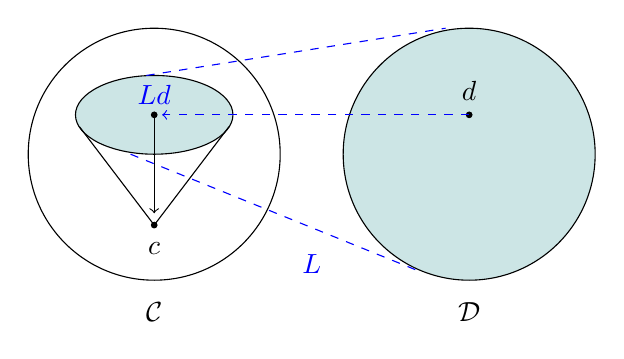
\begin{tikzpicture}
  \def\Xa{2.0};
  \def\Xb{-2.0};
  
  \def\Ytip{-0.9};
  \def\Yo{0.5}; % oval
  \def\Yb{-2.0}; % labels
         \draw (\Xa, 0)[fill=blue!50!green!20]  ellipse (1.6 and 1.6);
         \draw (\Xb , 0) ellipse (1.6 and 1.6);
         % oval
         \draw (\Xb , \Yo)[fill=blue!50!green!20] ellipse (1 and 0.5);
         
        % apex
        \filldraw (\Xb, \Ytip) circle (1pt);
        \node at ( \Xb, \Ytip - 0.3) { $c$ };
        
        % image
        \filldraw (\Xa, \Yo) circle (1pt);
        \node at ( \Xa, \Yo + 0.3) { $d$ };
        
	% middle of the cone
	\draw[->] (\Xb, \Yo) -- (\Xb, \Ytip + 0.15);
        	% sides of the cone
	\draw (\Xb, \Ytip) -- (\Xb + 0.95, \Yo - 0.15);
	\draw (\Xb, \Ytip) -- (\Xb - 0.95, \Yo - 0.15);

        % categories
        \node at (\Xa, \Yb) { $\mathcal D$ };
        \node at (\Xb, \Yb) { $\mathcal C$ };
        \node[blue] at (0, \Yb + 0.6) { $L$ };

        % functor middle
        \filldraw (\Xb, \Yo) circle (1pt);
        \node[blue] at ( \Xb, \Yo + 0.25) { $L d$ };
	\draw[->, blue, dashed] (\Xa, \Yo) -- (\Xb + 0.1, \Yo);
	% functor 
	\draw [blue, dashed] (\Xb - 0.1, \Yo + 0.5    )   --   (\Xa - 0.3, \Yo + 1.1);
	\draw [blue, dashed] (\Xb - 0.3, \Yo - 0.5) -- (\Xa - 0.6, \Ytip - 0.6);
\end{tikzpicture}
\]

The important observation is that this comma category describes a cocone in $\cat C$. The base of this cocone is formed by those objects in the image of $L$ that have an unobstructed view of $c$. The arrows in the base of the cocone are the morphisms in $L/c$. These are exactly the arrows that make the sides of the cocone commute.
\[
 \begin{tikzcd}
 L d
 \arrow[rd, "f"']
 \arrow[rr, "L h"]
 && L d'
 \arrow[ld, "f'"]
 \\
 &c
  \end{tikzcd}
 \hspace{30pt}
\begin{tikzcd}
 d
 \arrow[rr, "h"]
 && d'
  \end{tikzcd}
\]

The base of this cocone can then be projected back to $\cat D$. There is a projection $\pi_c$ which maps every pair $(d, f)$ in  $L/c$ back to $d$, thus forgetting the arrow $f$. It also maps every morphism in $L/c$ to an arrow in $\cat D$ that gave rise to it. This way $\pi_c$ defines a diagram in $\cat D$. The colimit of this diagram exists, because we have assumed that all colimits exist in $\cat D$. Let's call this colimit $t_c$:
\[ t_c = \text{colim}\; \pi_c \]

\[
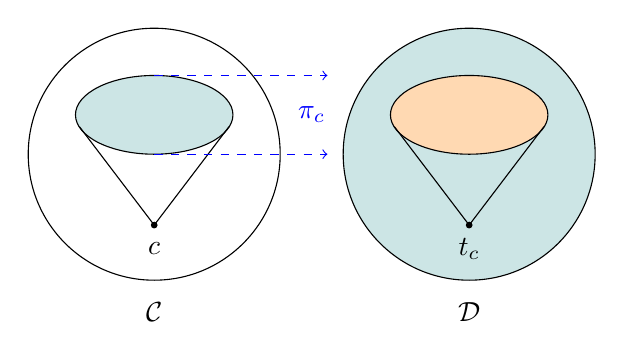
\begin{tikzpicture}
  \def\Xa{2.0};
  \def\Xb{-2.0};
  
  \def\Ytip{-0.9};
  \def\Yo{0.5}; % oval
  \def\Yb{-2.0}; % labels
         \draw (\Xa, 0)[fill=blue!50!green!20]   ellipse (1.6 and 1.6);
         \draw (\Xb , 0) ellipse (1.6 and 1.6);
         % oval
         \draw (\Xb , \Yo)[fill=blue!50!green!20]  ellipse (1 and 0.5);

        % apex
        \filldraw (\Xb, \Ytip) circle (1pt);
        \node at ( \Xb, \Ytip - 0.3) { $c$ };
                
        	% sides of the cone
	\draw (\Xb, \Ytip) -- (\Xb + 0.95, \Yo - 0.15);
	\draw (\Xb, \Ytip) -- (\Xb - 0.95, \Yo - 0.15);

         % second oval
         \draw (\Xa , \Yo) [fill=orange!30]  ellipse (1 and 0.5);
          
        % apex
        \filldraw (\Xa, \Ytip) circle (1pt);
        \node at ( \Xa, \Ytip - 0.3) { $t_c$ };

        	% sides of the cone
	\draw (\Xa, \Ytip) -- (\Xa + 0.95, \Yo - 0.15);
	\draw (\Xa, \Ytip) -- (\Xa - 0.95, \Yo - 0.15);

        % categories
        \node at (\Xa, \Yb) { $\mathcal D$ };
        \node at (\Xb, \Yb) { $\mathcal C$ };
        \node[blue] at (0, \Yo) { $\pi_c$ };

	% functor 
	\draw [->, blue, dashed] (\Xb, \Yo + 0.5) --  (\Xb + 2.2, \Yo + 0.5);
	\draw [->, blue, dashed] (\Xb, \Yo - 0.5)  -- (\Xb + 2.2, \Yo - 0.5);
\end{tikzpicture}
\]

Let's see if we can use this $t_c$ to construct a terminal object in $L/c$. We have to find an arrow, let's call it $\varepsilon_c \colon L t_c \to c$, such that the pair $\langle t_c, \varepsilon_c \rangle$ is terminal in $L/c$. 

Notice that $L$ maps the diagram generated by $\pi_c$ back to the base of the cocone defined by $L/c$. The projection $\pi_c$ did nothing more than to ignore the sides of this cocone, leaving its base intact. 

We now have two cocones in $\cat C$ with the same base: the original one with the apex $c$ and the new one obtained by applying $L$ to the cocone in $\cat D$. Since $L$ preserves colimits, the colimit of the new cocone is $L t_c$---the image of the colimit $t_c$:

\[ \text{colim} \; (L \circ \pi_c) = L ( \text{colim} \; \pi_c) = L t_c\]

By universal construction, we deduce that there must be a unique cocone morphism from the colimit $L t_c$ to $c$. That morphism, which we'll call $\varepsilon_c$, makes all the relevant triangles commute. 

What remains to be shown is that $\langle t_c, \varepsilon_c \rangle$ is terminal in $L/c$, that is, for any  $\langle d, f \colon L d \to c \rangle$ there is a unique comma-category morphism $h \colon d \to t_c$ that makes the following triangle commute:

\[
 \begin{tikzcd}
 L d
 \arrow[rd, "f"']
 \arrow[rr, dashed, "L h"]
 && L t_c
 \arrow[ld, red, "\varepsilon_c"]
 \\
 &c
  \end{tikzcd}
\]

Notice that any such $d$ is automatically part of the diagram produced by $\pi_c$ (it's the result of $\pi_c$ acting on $\langle d, f \rangle$). We know that $t_c$ is the limit of the $\pi_c$ diagram. So there must be a wire from $d$ to $t_c$ in the limiting cocone. We pick this wire as our $h$. 

\[
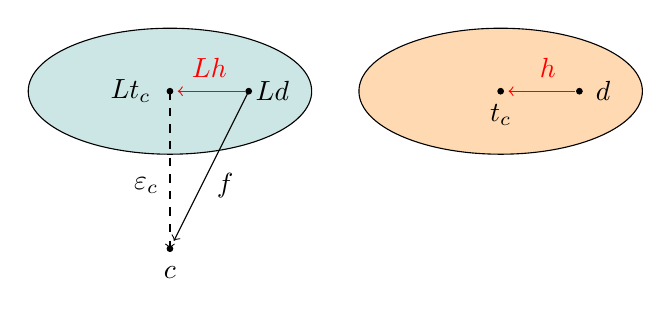
\begin{tikzpicture}
  \def\Xa{2.1};
  \def\Xb{-2.1};
  
  \def\Ytip{0};
  \def\Ybot{-2};
  \def\Yo{0}; % oval
  \def\Yf{-1.2}; % label
         % first oval
         \draw (\Xb , \Yo)[fill=blue!50!green!20]  ellipse (1.8 and 0.8);

         % second oval
         \draw (\Xa , \Yo) [fill=orange!30]  ellipse (1.8 and 0.8);
          
        % apex L tc
        \filldraw (\Xb, \Ytip) circle (1pt);
        \node at ( \Xb - 0.5, \Ytip) { $L t_c$ };
        
        % apex c
        \filldraw (\Xb, \Ybot) circle (1pt);
        \node at ( \Xb, \Ybot - 0.3) { $c$ };
                
        	% sides of the cone L h
	\draw[red, ->]  (\Xb + 0.95, \Yo) -- (\Xb + 0.1, \Ytip);
	\node[red] at (\Xb + 0.5, \Ytip + 0.3) {$L h$};

        % apex tc
        \filldraw (\Xa, \Ytip) circle (1pt);
        \node at ( \Xa, \Ytip - 0.3) { $t_c$ };

        	% sides of the cone h
	\draw [->, red] (\Xa + 0.95, \Yo) -- (\Xa + 0.1, \Ytip);
	\node[red] at ( \Xa + 0.6, \Ytip + 0.3) { $h$ };
	
	% d
        \filldraw (\Xa + 1, \Yo) circle (1pt);
        \node at ( \Xa + 1.3, \Yo) { $d$ };

	% L d
        \filldraw (\Xb + 1, \Yo) circle (1pt);
        \node at ( \Xb + 1.3, \Yo) { $L d$ };
        
        % f
        \draw[->] (\Xb + 1, \Yo) to (\Xb + 0.05, \Ybot + 0.1);
        \node at (\Xb + 0.7, \Yf) {$f$};
        
        % epsilon
        \draw[->, dashed] (\Xb, \Ytip) -- (\Xb, \Ybot);
        \node at (\Xb - 0.3, \Yf) {$\varepsilon_c$};

\end{tikzpicture}
\]
The commuting condition then follows from $\varepsilon_c$ being a morphism between two cocones. It is a unique cocone morphism simply because $\cat D$ is a preorder.

This proves that there is a universal arrow $\langle t_c, \varepsilon_c \rangle$ for every $c$, therefore we have a functor $R$ defined on objects as $R c = t_c$ that is the right adjoint to $L$.

\subsection{Solution set condition}

The problem with the previous proof is that comma categories in most practical cases are large: their objects don't form a set. But maybe we can approximate the comma category by selecting a smaller but representative set of objects and arrows?

To select the objects, we'd use a mapping from some indexing set $I$. We define a set of objects $d_i$ where $i \in I$. Since we are trying to approximate the comma category $L/c$, we select objects together with arrows $f_i \colon L d_i \to c$. 

The relevant part of the comma category is encoded in morphism between objects satisfying the commuting condition. We could try to specialize this condition to only apply inside our family of objects, but that would not be enough. We have to find a way to probe all other objects of the comma category. 

To do this, we reinterpret the commuting condition as a recipe for factorizing an arbitrary $f \colon L d \to c$ through some pair $\langle d_i, f_i \rangle$:
\[
 \begin{tikzcd}
 L d
 \arrow[rd, "f"']
 \arrow[rr, "L h"]
 && \textcolor{red}{L d_i}
 \arrow[ld, red, "f_i"]
 \\
 &c
  \end{tikzcd}
\]

A \index{solution set}\emph{solution set} is a family of pairs $\langle d_i, f_i \colon L d_i \to c \rangle $ indexed by a set $I$ that can be used to factor any pair $\langle d, f \colon L d \to c \rangle $. It means that there exists an index $i \in I$ and an arrow $h \colon d \to d_i$ that factorizes $f$:
\[ f = f_i \circ L h \]

Another way of expressing this property is to say that there exists a \index{weakly terminal set}\emph{weakly terminal} set of object in the comma category $L/c$. A weakly terminal set has the property that for any object in the category there is a morphism to at least one object in the set.

Previously we've seen that having the terminal object in the comma category $L/c$ for every $c$ is enough to define the adjunction. It turns out that we can achieve the same goal using the solution set. 

The assumptions of the Freyd's adjoint functor theorem state that we have a colimit-preserving functor $L \colon \cat D \to \cat C$ from a small co-complete category. Both these conditions relate to \emph{small} diagrams. If we can pick a solution set $\langle d_i, f_i \colon L d_i \to c \rangle $ for every $c$, then the right adjoint $R$ exists. Solution sets for different $c$'s may be different.

We've seen before that in a cocomplete category the existence of a weakly terminal set is enough to define a terminal object. In our case it means that, for any $c$, we can construct the universal arrow from $L$ to $c$. And this is enough to define the whole adjunction.

A dual version of the adjoint functor theorem can be used to construct the left adjoint.

\subsection{Defunctionalization}

Every programming language lets us define functions, but not all languages support higher level functions (functions taking functions as arguments, functions returning functions, or data types constructed from functions) or anonymous functions (a.k.a., lambdas). It turns out that, even in such languages, higher order functions can be implemented using the process called defunctionalization. This technique is based on the adjoint functor theorem. Moreover, defunctionalization can be used whenever passing functions around is impractical, for instance in a distributed system.

The idea behind defunctionalization is that the function type is defined as the right adjoint to the product. 
\[ \cat C(e \times a, b) \cong \cat C(e, b^a) \]
The adjoint functor theorem can be used to approximate this adjoint. 

In general, any finite program can only have a finite number of function definitions. These functions (together with the environments they capture) form the solution set that we can use to construct the function type. In practice, we do it only for a small subset of functions which occur as arguments to, or are returned from, other functions.

A typical example of the usage of higher order functions is in continuation passing style. For instance, here's a function that calculates the sum of the elements of a list. But instead of returning the sum it calls a continuation \hask{k} with the result:
\begin{haskell}
sumK :: [Int] -> (Int -> r) -> r
sumK [] k = k 0
sumK (i : is) k =
  sumK is (\s -> k (i + s))
\end{haskell}
If the list is empty, the function calls the continuation with zero. Otherwise it calls itself recursively, with two arguments: the tail of the list \hask{is}, and a new continuation:
\begin{haskell}
\s -> k (i + s)
\end{haskell}
This new continuation calls the previous continuation \hask{k}, passing it the sum of the head of the list and its argument \hask{s} (which is the accumulated sum). 

Notice that this lambda is a closure: It's a function of one variable \hask{s}, but it also has access to \hask{k} and \hask{i} from its environment.

To extract the final sum, we call our recursive function with the trivial continuation, the identity:
\begin{haskell}
sumList :: [Int] -> Int
sumList as = sumK as (\i -> i)
\end{haskell}

Anonymous functions are convenient, but nothing prevents us from using named functions. However, if we want to factor out the continuations, we have to be explicit about passing in the environments. 

For instance, we can replace our first lambda:
\begin{haskell}
\s -> k (i + s)
\end{haskell}
with the function \hask{more}, but we have to explicitly pass the pair \hask{(i, k)} as the environment of the type \hask{(Int, Int -> r)}:
\begin{haskell}
more :: (Int, Int -> r) -> Int -> r
more (i, k) s = k (i + s)
\end{haskell}
The other lambda, the identity, uses the empty environment, so it becomes:
\begin{haskell}
done :: Int -> Int
done i = i
\end{haskell}
Here's the implementation of our algorithm using these two named functions:
\begin{haskell}
sumK' :: [Int] -> (Int -> r) -> r
sumK' [] k = k 0
sumK' (i : is) k =
  sumK' is (more (i, k))
\end{haskell}

\begin{haskell}
sumList :: [Int] -> Int
sumList is = sumK' is done
\end{haskell}

In fact, if all we are interested in is calculating the sum, we can replace the polymorphic type \hask{r} with \hask{Int} with no other changes.

This implementation still uses higher order functions. In order to eliminate them, we have to analyze what it means to pass a function as an argument. Such a function can only be used in one way: it can be applied to its arguments. This property of a function type is expressed as the counit of the currying adjunction:
\[ \varepsilon \colon b^a \times a \to b \]
or, in Haskell, as a higher-order function:
\begin{haskell}
apply :: (a -> b, a) -> b
\end{haskell}
This time we are interested in constructing the counit from first principles. We've seen that this can be accomplished using the comma category. In our case, an object of the comma category for the product functor $L_a = (-) \times a$ is a pair 
\[(e, f \colon (e \times a) \to b) \]
or, in Haskell:
\begin{haskell}
data Comma a b e = Comma e ((e, a) -> b)
\end{haskell}
A morphism in this category between $(e, f)$ and $(e', f')$ is an arrow $h \colon e \to e'$, which satisfies the commuting condition:
\[ f' \circ h = f \]
We interpret this morphism as ``reducing'' the environment $e$ down to $e'$. The arrow $f'$ is able to produce the same output of the type $b$ using a potentially smaller environment given by $h (e)$. For instance $e$ may contain variables that are irrelevant for computing $b$ from $a$, and $h$ projects them out. 

\[
 \begin{tikzcd}
 e \times a
 \arrow[rd, "f"']
 \arrow[rr, "h \times a"]
 && e' \times a
 \arrow[ld, "f'"]
 \\
 &b
  \end{tikzcd}
 \hspace{30pt}
\begin{tikzcd}
 e
 \arrow[rr, "h"]
 && e'
  \end{tikzcd}
\]


In fact, we performed this kind of reduction when defining \hask{more} and \hask{done}. In principle, we could have passed the tail \hask{is} to both functions, since it's accessible at the point of call. But we knew that they didn't need it.

Using the Freyd's theorem, we could define the function object $a \to b$ as the colimit of the diagram defined by the comma category. Such a colimit is essentially a giant coproduct of all environments modulo identifications given by comma-category morphisms. This identification does the job of reducing the environment needed by $a \to b$ to the bare minimum. 

In our example, the continuations we're interested in are functions \hask{Int -> Int}. In fact we are not interested in generating the generic function type \hask{Int -> Int}; just the minimal one that would accommodate our two functions \hask{more} and \hask{done}. We can do it by creating a very small solution set. 

In our case the solution set consists of pairs $(e_i, f_i \colon e_i \times a \to b)$ such that any pair $(e, f \colon e \times a \to b)$ can be factorized through one of the $f_i$'s. More precisely, the only two environments we're interested in are \hask{(Int, Int ->Int)} for \hask{more}, and the empty environment \hask{()} for \hask{done}. 

In principle, our solution set should allow for the factorization of every object of the comma category, that is a pair of the type:
\begin{haskell}
(e, (e, Int) -> Int)
\end{haskell}
but here we are only interested in two specific functions. Also, we are not concerned with the uniqueness of the representation so, instead of using a colimit (as we did for the adjoint functor theorem), we'll just use a coproduct of all the environments of interest. We end up with the following data type that is the sum of the two environments, \hask{()} and \hask{(Int, Int -> Int)}, we're interested in. We end up with the type:
\begin{haskell}
data Kont = Done | More Int Kont
\end{haskell}
Notice that we have recursively encoded the \hask{Int->Int} part of the environment as \hask{Kont}. Thus we have also removed the need to use functions as arguments to data constructors.

If you look at this definition carefully, you will discover that it's the definition of a list of \hask{Int}, modulo some renamings. Every call to \hask{More} pushes another integer on the \hask{Kont} stack. This interpretation agrees with our intuition that recursive algorithms require some kind of a runtime stack. 

We are now ready to implement our approximation to the counit of the adjunction. It's composed from the bodies of the two functions, with the understanding that recursive calls also go through \hask{apply}:
\begin{haskell}
apply :: (Kont, Int) -> Int
apply (Done, i) = i
apply (More i k, s) = apply (k, i + s)
\end{haskell}
Compare this with our earlier:
\begin{haskell}
done i = i
more (i, k) s = k (i + s)
\end{haskell}


The main algorithm can now be rewritten without any higher order functions or lambdas:
\begin{haskell}
sumK'' :: [Int] -> Kont -> Int
sumK'' [] k = apply (k, 0)
sumK'' (i : is) k = sumK'' is (More i k)
\end{haskell}

\begin{haskell}
sumList'' is = sumK'' is Done
\end{haskell}

The main advantage of defunctionalization is that it can be used in distributed environments. Arguments to remote functions, as long as they are data structures and not functions, can be serialized and sent along the wire. All that's needed is for the receiver to have access to \hask{apply}. 

\section{Free/Forgetful Adjunctions}
The two functors in the adjunction play different roles: the picture of the adjunction is not symmetric. Nowhere is this illustrated better than in the case of the free/forgetful adjunctions. 

A forgetful functor is a functor that ``forgets'' some of the structure of its source category. This is not a rigorous definition but, in most cases, it's pretty obvious what structure is being forgotten. Very often the target category is just the category of sets, which is considered the epitome of structurelessness. The result of the forgetful functor in that case is called the ``underlying'' set, and the functor itself is often called $U$. 

More precisely, we say that a functor forgets \emph{structure} if the mapping of hom-sets is not surjective, that is, there are arrows in the target hom-set that have no corresponding arrows in the source hom-set. Intuitively, it means that the arrows in the source have some structure to preserve, so there are fewer of them; and that structure is absent in the target. 

The left adjoint to a forgetful functor is called a \emph{free functor}.

\[
 \begin{tikzcd}
F x
\arrow[d, bend right, red, dashed]
\arrow[d, dashed]
\arrow[d, bend left, blue, dashed]
  &&
  x
\arrow[d, bend right, red, dashed]
\arrow[d, dashed]
\arrow[d, bend left, blue, dashed]
 \arrow[ll, bend right, "F"']
 \\
y
   \arrow[rr, bend right, "U"']
 &&
 U y
  \end{tikzcd}
\]

A classic example of a free/forgetful adjunction is the construction of the free monoid.


\subsection{The category of monoids}
Monoids in a monoidal category $\mathcal{C}$ form their own category $\mathbf{Mon}(\mathcal{C})$. Its objects are monoids, and its arrows are the arrows of $\mathcal{C}$ that preserve the monoidal structure. 

The following diagram explains what it means for $f$ to be a monoid morphism, going from a monoid $(M_1, \eta_1, \mu_1)$ to a monoid $(M_2, \eta_2, \mu_2)$:
\[
 \begin{tikzcd}
 & M_1
 \arrow[dd, "f"]
 & M_1 \otimes M_1
 \arrow[l, "\mu_1"]
 \arrow[dd, "f \otimes f"]
 \\
 I
 \arrow[ru, "\eta_1"]
 \arrow[rd, "\eta_2"']
 \\
 & M_2
 & M_2 \otimes M_2
 \arrow[l, "\mu_2"]
  \end{tikzcd}
\]
A monoid morphism $f$ must map unit to unit, which means that:
\[ f \circ \eta_1 = \eta_2 \]
and it must map multiplication to multiplication:
\[ f \circ \mu_1 = \mu_2 \circ (f \otimes f)\]
Remember, the tensor product $\otimes$ is functorial, so it can lift pairs of arrows, as in $f \otimes f$.

In particular, the category $\mathbf{Set}$ is monoidal, with cartesian product and the terminal object providing the monoidal structure. 

In particular, monoids in $\mathbf{Set}$ are sets with additional structure. They form their own category $\mathbf{Mon}(\mathbf{Set})$ and there is a forgetful functor $U$ that simply maps the monoid to the set of its elements. When we say that a monoid is a set, we mean the underlying set.

\subsection{Free monoid}

We want to construct the free functor 
\[ F \colon \mathbf{Set} \to \mathbf{Mon}(\mathbf{Set})\]
that is adjoint to the forgetful functor $U$. 

We start with an arbitrary set $X$ and an arbitrary monoid $m$. On the right-hand side of the adjunction we have the set of functions from $X$ to $U m$. On the left-hand side, we have a set of highly constrained structure-preserving monoid morphisms from $F X$ to $m$. How can these two hom-sets be isomorphic?

In  $\mathbf{Mon}(\mathbf{Set})$, monoids are sets of elements, and monoid morphisms are functions between such sets, satisfying additional constraints: preserving unit and multiplication. 

Arrows in $\mathbf{Set}$, on the other hand, are just functions with no additional constraints. So, in general, there are fewer arrows between monoids than there are between their underlying sets. 

\[
 \begin{tikzcd}
F X
\arrow[d, bend right, red, dashed]
\arrow[d, dashed]
\arrow[d, bend left, blue, dashed]
  &&
X
\arrow[d, bend right, red, dashed]
\arrow[d, dashed]
\arrow[d, bend left, blue, dashed]
 \arrow[ll, bend right, "F"']
 \\
m
   \arrow[rr, bend right, "U"']
 &&
 U m
  \end{tikzcd}
\]

Here's the idea: if we want to have a one to one matching between arrows, we want $F X$ to be much larger than $X$. This way, there will be many more functions from it to $m$---so many that, even after rejecting the ones that don't preserve the structure, we'll still have enough to match every function $f \colon X \to U m$.

We'll construct the monoid $F X$ starting from the set $X$, and adding more and more elements as we go. We'll call the initial set $X$ the \index{generators of a monoid}\emph{generators} of $F X$. We'll construct a monoid morphism $g \colon F X \to m$ starting with the original function $f$ and extending it to act on more and more elements.

On generators, $x \in X$, $g$ works the same as $f$:
\[ g x = f x \]

Since $F X$ is supposed to be a monoid, it has to have a unit. We can't pick one of the generators to be the unit, because it would impose constraints on the part of $g$ that is already fixed by $f$---it would have to map it to the unit $e'$ of $m$. So we'll just add an extra element $e$ to $F X$ and call it the unit. We'll define the action of $g$ on it by saying that it is mapped to the unit $e'$ of $m$:
\[ g e = e' \]

We also have to define monoidal multiplication in $F X$. Let's start with a product of two generators $a$ and $b$. The result of the multiplication cannot be another generator because, again, that would constrain the part of $g$ that's fixed by $f$---products must be mapped to products. So we have to make all products of generators new elements of $F X$. Again, the action of $g$ on those products is fixed:
\[ g (a \cdot b)  = g a \cdot g b\]

Continuing with this construction, any new multiplication produces a new element of $F X$, except when it can be reduced to an existing element by applying monoid laws. For instance, the new unit $e$ times a generator $a$ must be equal to $a$. But we have made sure that $e$ is mapped to the unit of $m$, so the product $g e \cdot g a$ is automatically equal to $g a$.

Another way of looking at this construction is to think of the set $X$ as an alphabet. The elements of $F X$ are then strings of characters from this alphabet. The generators are single-letter strings, ``$a$'', ``$b$'', and so on. The unit is an empty string ``''. Multiplication is string concatenation, so  ``$a$'' times ``$b$'' is a new string ``$ab$''. Concatenation is automatically associative and unital, with the empty string as the unit.

The intuition behind free functors is that they generate structure ``freely,'' as in ``with no additional constraints.'' They also do it lazily: instead of performing operations, they just record them. They create generic domain-specific programs that can be executed later by specific interpreters.

The free monoid ``remembers to do the multiplication'' at a later time. It stores the arguments to multiplication in a string, but doesn't perform the multiplication. It's only allowed to simplify its records based on generic monoidal laws. For instance, it doesn't have to store the command to multiply by the unit. It can also ``skip the parentheses'' because of associativity. 

\begin{exercise}
What is the unit and the counit of the free monoid adjunction $F \dashv U$?
\end{exercise}

\subsection{Free monoid in programming}

In Haskell, monoids are defined using the following typeclass:
\begin{haskell}
class Monoid m where
  mappend :: m -> m -> m
  mempty  :: m
\end{haskell}
Here, \hask{mappend} is the curried form of the mapping from the product: \hask{(m, m) -> m}. The \hask{mempty} element corresponds to the arrow from the terminal object (unit of the monoidal category), or simply an element of \hask{m}. 

A free monoid generated by some type \hask{a}, which serves as a set of generators, is represented by a list type \hask{[a]}. An empty list serves as the unit; and monoid multiplication is implemented as list concatenation, traditionally written in infix form:
\begin{haskell}
(++) :: [a] -> [a] -> [a]
(++) []     ys = ys
(++) (x:xs) ys = x : xs ++ ys
\end{haskell}
A list is an instance of a \hask{Monoid}:
\begin{haskell}
instance Monoid [a] where
  mempty = []
  mappend = (++)
\end{haskell}

To show that it's a free monoid, we have to be able to construct a monoid morphism from the list of \hask{a} to an arbitrary monoid \hask{m}, provided we have an (unconstrained) mapping from \hask{a} to (the underlying set of) \hask{m}. We can't express all of this in Haskell, but we can define the function:
\begin{haskell}
foldMap :: Monoid m => (a -> m) -> ([a] -> m)
foldMap f = foldr mappend mempty . fmap f
\end{haskell}
This function transforms the elements of the list to monoidal values using \hask{f} and then folds them using \hask{mappend}, starting with the unit \hask{mempty}. 

It's easy to see that an empty list is mapped to the monoidal unit. It's not too hard to see that a concatenation of two lists is mapped to the monoidal product of the results. So, indeed, \hask{foldMap} is a monoid morphism. 

Following the intuition of a free monoid being a domain-specific program for multiplying stuff, \hask{foldMap} provides an \emph{interpreter} for this program. It performs all the multiplications that have been postponed. Note that the same program may be interpreted in many different ways, depending on the choice of the concrete monoid and the function \hask{f}.

We'll come back to free monoids as lists in the chapter on algebras.

\begin{exercise}
Write a program that takes a list of integers and interprets it in two different ways: once using the additive and once using the multiplicative monoid of integers.
\end{exercise}

\section{The Category of Adjunctions}
We can define composition of adjunctions by taking advantage of the composition of functors that define them. Two adjunctions, $L \dashv R$ and $L' \dashv R'$, are composable if they share the category in the middle:
\[
 \begin{tikzcd}
  \mathcal{C}
  \arrow[rr, bend right, "R'"']
  &&
  \mathcal{D}
  \arrow[ll, bend right, "L'"']
    \arrow[rr, bend right, "R"']
&&
  \mathcal{E}
  \arrow[ll, bend right, "L"']
 \end{tikzcd}
\]
By composing the functors we get a new adjunction $(L' \circ L) \dashv (R \circ R')$. 

Indeed, let's consider the hom-set:
\[ \mathcal{C}(L' (L e), c) \]
Using the $L' \dashv R'$ adjunction, we can transpose $L'$ to the right, where it becomes $R'$:
\[ \mathcal{D}(L e, R' c) \]
and using $L \dashv R$ we can similarly transpose $L$:
\[ \mathcal{E}( e, R(R' c)) \]
Combining these two isomorphisms, we get the composite adjunction:
\[ \mathcal{C}((L' \circ L) e, c) \cong \mathcal{E}( e, (R \circ R') c)\]

Because functor composition is associative, the composition of adjunctions is also associative. It's easy to see that a pair of identity functors forms a trivial adjunction that serves as the identity with respect to composition of adjunctions. Therefore we can define a category $\mathbf{Adj}(\mathbf{Cat})$ in which objects are categories and arrows are adjunctions (by convention, pointing in the direction of the left adjoint). 

Adjunctions can be defined purely in terms of functors and natural transformations, that is 1-cells and 2-cells in the 2-category $\mathbf{Cat}$. There is nothing special about $\mathbf{Cat}$, and in fact adjunctions can be defined in any 2-category. Moreover, the category of adjunctions is itself a 2-category.

\section{Levels of Abstraction}

Category theory is about structuring our knowledge. In particular, it can be applied to the knowledge of category theory itself. Hence we see a lot of mixing of abstraction levels in category theory. The structures that we see at one level can be grouped into higher-level structures which exhibit even higher levels of structure, and so on. 

In programming we are used to building hierarchies of abstractions. Values are grouped into types, types into kinds. Functions that operate on values are treated differently than functions that operate on types. We often use different syntax to separate levels of abstractions. Not so in category theory.

A set, categorically speaking, can be described as a discrete category. Elements of the set are objects of this category and, other than the obligatory identity morphisms, there are no arrows between them. 

The same set can then be seen as an object in the category $\mathbf{Set}$. Arrows in this category are functions between sets.

The category $\mathbf{Set}$, in turn, is an object in the category $\mathbf{Cat}$. Arrows in $\mathbf{Cat}$ are functors. 

Functors between any two categories $\mathcal{C}$ and $\mathcal{D}$ are objects in the functor category $[\mathcal{C}, \mathcal{D}]$. Arrows in this category are natural transformations.

We can define functors between functor categories, product categories, opposite categories, and so on, ad infinitum. 

Completing the circle, hom-sets in every category are sets. We can define mappings and isomorphisms between them, reaching across disparate categories. Adjunctions are possible because we can compare hom-sets that live in different categories.

\end{document}